\section{FAST raksturpunktu noteikšanas algoritms} \label{sec:fast}
\setcounter{lstlisting}{0} %Reset listings counter (for the section)

\newcommand{\Ip}{I_{\vec{p}}}
\newcommand{\Ipc}{ {I_{\vec{p} \to c}} }
\newcommand{\Spc}{ {S_{\vec{p} \to c}} }

% TODO?: Nodaļas ievads?
\subsection{Definīcija} \label{sec:fast-def}
\subsubsection{Punktu klasifikācija}

\begin{figure}[tbh]
	\centering
	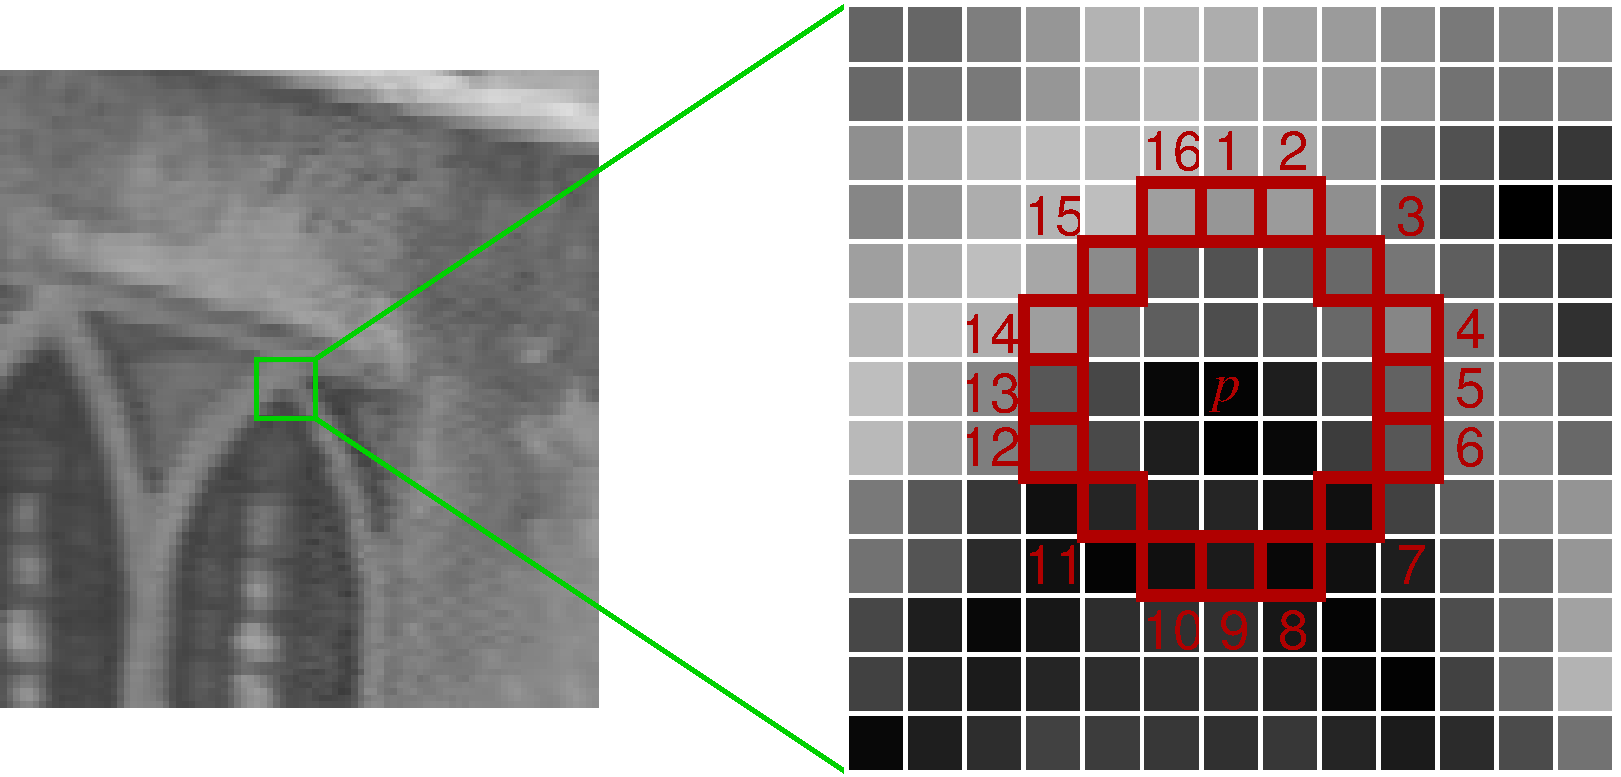
\includegraphics[width=0.7\textwidth]{fast-corner}
	\caption{FAST 16 pikseļu riņķa pārbaudes logs~\cite{FAST}.}
	\label{fig:fast}
\end{figure}

FAST ir Rostena~un~Dramonda\cite{FAST}~(\termEn{Rosten and Drummond})
izstrādāts stūru detektors, kurš tiek izmantots attēla potenciālo 
raksturpunktu noteikšanai~(sk.~\ref{sec:corners}~nod.).

FAST detektors kandidāta punkta $\vec{p}$ klasificēšanai, izmanto intensitāšu
salīdzināšanu starp punktu $\vec{p}$ un 16~pikseļu riņķi (\termEn{Bresenham} riņķis
ar rādiusu 3) ap punktu $\vec{p}$. 
FAST definīcija nosaka, ka apskatāmais punkts $\vec{p}$ ir uzskatāms par
,,stūri'' tad, ja $n$ skaita secīgi pikseļi ir, vai nu gaišāki
(ar augstāku intensitāte) par kandidāta pikseļa intensitāti $\Ip$, kuram
pieskaitīta sliekšņa vērtība $t$, vai tumšāki (ar zemāku intensitāte) par
$\Ip - t$. \cite{Rosten-tracking}\cite{FAST}

Katrs no riņķa punktiem, kurus apzīmēsim ar $\vec{p}\to c$, kur $c \in [1; 16]$,
var būt vienā no trīs stāvokļiem:
\begin{equation}\label{eq:fast}
	\Spc := \left\{
		\begin{array}{c}
			d\text{,}\quad\text{ja}\\
			s\text{,}\quad\text{ja}\\
			b\text{,}\quad\text{ja}
		\end{array}
		\begin{aligned}
			           & \Ipc < \Ip-t \\
			\Ip-t \leq & \Ipc \leq \Ip+t \\
			   \Ip+t < & \Ipc
		\end{aligned}
		\right.
\end{equation}
kur $d$ un $b$ attiecīgi apzīmē ,,tumšāks'' vai ,,gaišāks'', un $s$ apzīmē
,,līdzīgs''. Tātad $n$ skaitam $\Spc$ vērtību ar secīgiem $c$ jābūt visiem
$b$ stāvoklī, vai visiem $d$ stāvoklī, lai $\vec{p}$ tiktu klasificēts kā
,,stūra'' punkts. Šajā pielietojumā visi atrastie ,,stūri'' tiek pieņemti
par attēla raksturpunktiem.

Uzdotā \eqref{eq:fast} definīcija ir autora koriģēta, jo ir novērota pretruna
Rostena un~Dramonda\cite{FAST} definīcijā pret visu apskatīto
FAST implementāciju (t.sk.~Rostena un Dramonda\cite{FAST} pašu implementācijas)
funkcionalitāti. Avotā \cite{FAST} stāvokļi $d$ un $b$ ir definēti ar
nestingrām nevienādībām, kaut gan visās implementācijās izmantota stingrā
salīdzināšana. Autors devis priekšroku implementāciju funkcionalitātei un
attiecīgi veicis korekcijas definīcijā.

Vienkāršākā šīs definīcijas algoritmiska implementācija ir, katram
punktam $\vec{p}$ secīgi pārbaudīt visus $c$ (nosakot $\Spc$)
līdz tiek konstatēti $n$ skaita punkti, kas atbilst iepriekšminētajam
kritērijam. Rostens~un~Dramonds\cite{FAST} šādu implementāciju sauc par
,,\emph{segmenta testu}''. Pilns segmenta tests ir uzskatāma par 
neefektīvu implementāciju~\cite{FAST},
un \ref{sec:fast-impl} nodaļā tiek apskatītas citi FAST implementāciju varianti.


\subsubsection{Lokālo maksimumu atlase}
FAST klasifikācijas rezultātā var rasties situācija, ka vairāki 
blakus esoši pikseļi tiek klasificēti kā raksturpunkti.
Raksturpunktu salāgošanai šī ir nevēlama situācija, jo šo punktu apkārtnes
ir līdzīgas un var radīt salāgošanas konfliktus.

Lai šo situāciju novērstu, izmanto lokālo maksimumu atlasi, kas lokalizētā
apkārtnē atstāj tikai punktu ar maksimālo vērtību, kā ilustrēts \ref{fig:nonmax}~attēlā.
Jāņem vērā, ka FAST
klasifikācija atgriež tikai bināru vērtību vai punkts ir ,,stūris'',
tādēļ nepieciešams piešķirt punktiem to kvantitatīvu ,,stūrainības'' mēru.

Lai gan \cite{FAST}~avotā ir definīcija, punktu vērtēšanai izmantojot
absolūto starpību summu, autors konstatē, ka publicētajā programmas pirmkodā%
\footnote{\url{http://www.edwardrosten.com/work/fast.html}}
neatbilst definīcijai.

%\begin{singlespace}
% NOTE: No Need for singlespace when floated!
	\lstinputlisting[language={C++},float=thb,%
	                 caption={,,Stūra'' punkta vērtēšanas funkcija~\cite{FASTER-src}.},%
	                 linerange={2915-2933},firstnumber=2915,%
	                 breaklines,breakatwhitespace,%
	                 label=kb:fast-score-cvd]
		{code/fast9.cc}
%\end{singlespace}

Pēc koda analīzes (sk.~\ref{kb:fast-score-cvd}~pirmkodu)
autors secina, ka punkti tiek vērtēti pēc sliekšņa $t$ vērtības
(pirmkodā mainīgais \texttt{b}), pie kuras
punkts joprojām atbilst ,,stūra'' kritērijam.

Formāli, ja FAST klasifikāciju uzdodam kā funkciju $F_n(\vec{p}, t)$,
kura ir patiesa, ja punkts $\vec{p}$ pie sliekšņa $t$ ir klasificējams
kā ,,stūris'', tad vērtības funkciju varam definēt kā:
\begin{equation}\label{eq:fast-response}
	V(\vec{p}) := \left\{ \max{t} : F_n(\vec{p}, t) \right\}
\end{equation}
Funkcionāli ekvivalenta realizācija izmantota visās apskatītajās FAST
implementācijās.

%~ Tika noskaidrots, ka FAST pirmkodā vērtēšanas funkcija izmainīta versijā~2.0,
%~ kas izlaista pēc \cite{FAST} avota publikācijas. Toties Rostena jaunākā
%~ publikācijā, jau aprakstīta izmainītā FAST punktu vērtēšana,
%~ bet nav minēts izmaiņas pamatojums~\cite{FASTER}.

\begin{figure}[tbh]
	\centering
	\def\svgwidth{0.8\linewidth}
	{\input{img/nonmax-suppression.pdf_tex}}
	\caption{Raksturpunktu klasifikācija un lokālo maksimumu atlase.}
	\label{fig:nonmax}
\end{figure}

Kad punkti ir klasificēti un rezultējošiem raksturpunktiem piekārtota
vērtība, tiek salīdzinātas vērtības blakusesošiem raksturpunktiem
jeb
noteikts lokālais maksimums $3 \times 3$ pikseļu logā katram
\phantomsection\label{sym:A}
$\vec{p} \in F_n(\vb{A}, t)$, kur $\vb{A}$ ir viss attēls.
Punkti, kuri nav lokālie maksimumi tiek atmesti no raksturpunktu kopas.
Rezultējošo kopu apzīmēsim ar $\hat{F_n}(\vb{I}, t)$.

FAST lokālo maksimumu atlasei tiek izmantoti divi varianti:
\begin{itemize}
	\item ,,\emph{relaksētais}'', kurš pieļauj blakusesošus, ja to
		vērtības ir vienādas (maksimuma vērtība ir nestingri lielāka), un
	\item ,,\emph{striktais}'', kur maksimuma vērtībai jābūt stingri
		lielākai par apkārtnes punktu vērtībām, pretējā gadījumā abi (vai
		visi) šie raksturpunkti tiek atmesti.
\end{itemize}
No abiem variantiem, autors izvēlējās un darbā izmanto ,,strikto'' definīciju,
jo varbūtība blakusesošiem raksturpunktiem, ka tiem sakritīs to
\termTech{deskriptori} salāgošanai, radot konfliktu, ir ļoti augsta.
Pie tam, pat ja tā nav, tad pozīcijas nenoteiktības dēļ, raksturpunkti tik
un tā ir uzskatāmi par nekvalitatīviem un ir nevēlami iekļaušanai
raksturpunktu kopā.

\subsection{Implementāciju modeļi} \label{sec:fast-impl}
\subsubsection{Oriģinālā FAST implementācija} \label{sec:fast-original}
\TODO

\subsubsection{OpenCV FAST impementācija (CPU)} \label{sec:fast-ocv}
OpenCV\footnote{\url{http://opencv.org/}} piedāvā alternatīvu FAST9 
(FAST ar $n=9$) algoritma
implementāciju (FAST ar citām $n$ vērtībām netiek implementētas)~\cite{OpenCV-src}.
Tās pamatā ir segmenta tests ar papildinātu
priekšpārbaudi\cite{Rosten-tracking}\cite{FAST}, kas var klasificēt vairumu
gadījumu, kad punkts $\vec{p}$ nav ,,stūris''. Priekšpārbaudi iztur
punkti kas ir ,,stūri'', jeb visi $\vec{p} \in F_9(\vb{I}, t)$,
un noteikta apakškopa punktu, kuri neatbilst $F_9(\vb{I}, t)$ un kuru
apkārtne ir ļoti specifiska un reālos attēlos ir statistiski reti.
Neskatoties
uz to, jebkuram punktam, kas iztur priekšpārbaudi, tiek veikts segmenta
tests, lai nodrošinātu pilnīgu klasifikāciju.
Var tikt veikts arī daļējs segmenta tests, jo priekšpārbaude var,
vairumā gadījumu, papildus noteikt vai ir meklējams ,,tumšs'' segments, vai
,,gaišs'' segments.

Šāda implementācija, ,,skalāra~koda\footnote{Kods, kas neizmanto SIMD
	instrukcijas, pretstatā ,,vektoriskam'' kodam.}''
izpildījumā, dod nelielu uzlabojumu. OpenCV implementācijas galvenā
priekšrocība ir SSE2 SIMD instrukciju izmantojums, kas ļauj vienlaikus
apstrādāt 16 kandidātu punktus (pikseļus). Empīriski novērotais
uzlabojums ir līdz 4 reizēm ātrāk (sk.~pielikumu~\ref{appx:test1})
par neapmācītu mašīnmācāmo implementāciju.

%~ \subsubsection*{OpenCL versija}
\subsubsection{OpenCV FAST impementācijas OpenCL versija (GPU)} \label{sec:fast-ocv-cl}
OpenCV piedāvā arī OpenCL FAST implementāciju izpildei GPU~\cite{OpenCV-src}.
Atšķirībā no CPU versijas, OpenCL implementē pilnu segmenta testu bez
priekšpārbaudes. Tas ir, galvenokārt, tādēļ, ka priekšpārbaudes loma ir
īsākā laikā konstatēt, ka apskatāmais punkts nav stūris un turpmākās pārbaudes
neveikt. Priekšpārbaude realizē zarošanos, kas degradē veiktspēju
nekoherentas zarošanās gadījumā (sk.~\ref{sec:gpu}~un \ref{sec:proc-cmp}~nod.).

Būtiska gan ir šīs implementācijas paralēlā darbība. Algoritms tiek
izpildīts divos secīgos etapos (atspoguļojot FAST definīciju):
\begin{enumerate}
	\item \emph{punktu klasifikācija}, kas pārbauda vai
		$\vec{p} \in F_9(\vb{I}; t)$, izveidojot izpildes pavedienu katram
		attēla punktam $\vec{p}$;
	\item \emph{lokālo maksimumu atlase}, kur atmetot raksturpunktus,
		kuri nav maksimumi $3 \times 3$ pikseļu logā atlasa apakškopu
		$\hat{F_9}(\vb{I}; t) \subseteq F_9(\vb{I}; t)$, izveidojot
		izpildes pavedienam katram klasificētajam raksturpunktam
		$\vec{p} \in F_9(\vb{I}; t)$.
\end{enumerate}

Interesanta implementācijas detaļa ir, ka lokālo maksimumu atlases solī
visiem punktiem $3 \times 3$ logā tiek aprēķināts stūra mērs,
nepārbaudot, vai tie ir klasificēti kā raksturpunkti iepriekšējā solī.
Šī pārbaude nav obligāta, jo stūru mērs $V(\vec{p})$ punktiem,
kas nav raksturpunkti ir vienmēr mazāks, un rezultāti ir identiski ar
CPU implementācijas rezultātiem.

GPU implementācijas ātrdarbība tika eksperimentāli salīdzināta ar CPU
implementāciju, bet tās ātrdarbība nepārsniedza CPU implementāciju
(sk.~pielikumu~\ref{appx:test2}).
Salīdzinājums izvērsts \ref{sec:fast-compare}~nodaļā.

\subsubsection{FAST FPGA implementācijas modelis} \label{sec:fast-fpga}
FAST potenciālās ātrdarbības salīdzināšanai FPGA platformai, autors
izstrādājis savu implementācijas modeli. Pēc vairākiem uzbūves variantiem,
%TODO?: Atmestie modeļi?
autors par piemērotāko atzinis modeli, kas balstās atsevišķu apstrādes
vienību izmantoto resursu samazināšanu, un caurlaidspējas palielināšanu
instancējot lielu skaitu šo vienību.

\begin{figure}[tbh]
	\centering
	\def\svgwidth{\linewidth}
	{\small\input{img/fpga-model.pdf_tex}}
	\caption{Vienkāršota uzbūves shēma viena punkta apstrādes vienībai.}
	\label{fig:fast-fpga}
\end{figure}

Tā kā viena elementa --- punkta $\vec{p}$ piederības $F_9(\vb{I},t)$ ---
noteikšanas latentums nav prioritāte, apstrādes vienība, kā ilustrēts
\ref{fig:fast-fpga}~attēlā, resursu ekonomijas nolūkos, ir secīgas uzbūves.
Salīdzināšana ar apkārtnes punktiem notiek secīgi, to intensitātes vērtības
pārvietojot caur bīdes reģistru un ar skaitītājiem uzskaitot secīgu
gaišo un tumšo loka punktu skaitu. Šāda FAST-9 apstrādes vienība vienu punktu
var klasificēt $16+(n-1)=24$ takts ciklos, bet papildus takts cikli
var būt nepieciešami datu sagatavošanai.

Katra FAST punkta apstrādes vienība tad var tikt instancēta un vairāki
punkti klasificēti paralēli. Testiem tika izveidots
,,attēlu apgabalu procesors'', kas vienlaikus apstrādā $w \times w$ attēla
apakškopu, kur ${(w-6)}^2$ punkta apstrādes instances klasificē attēla
apakškopas punktus. Sintēzes rezultāti uzrādīja CPU līdzvērtīgu ātrdarbību
izmantojot tikai 18\% Virtex-6 resursu
(sk.~pielikumu~\ref{appx:test3}).

\begin{figure}[tbh]
	\centering
	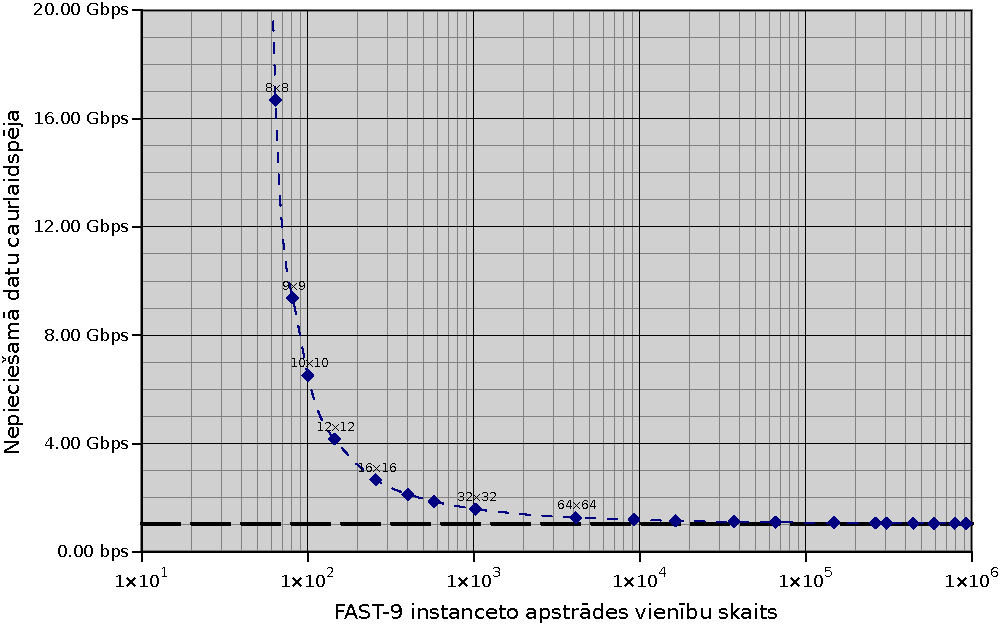
\includegraphics[scale=0.77]{chart-overhead}
	\caption{Caurlaidspējas virstēriņš pret FAST instanču skaitu.}
	\label{fig:overhead}
\end{figure}
Lai arī ,,attēla apgabalu procesors'' ir adekvāta konstrukcija
ātrdarbības pārbaudei, tika konstatēts, ka lielāku attēlu dalīšana
apstrādei gabalos, ļoti neefektīvi izmanto pieejamo caurlaidspēju, ja
netiek izmantoti atmiņas buferi pārklājošās informācijas saglabāšanai.
Caurlaidspējas \newTerm{virstēriņa} (\termEn{overhead}) apjoms ir atkarīgs no
izvēlētā $w$ --- virstēriņš strauji samazinās pie lielāka $w$,
kā redzams \ref{fig:overhead}~attēlā, kur ar melnu, pārtrauktu līniju
atzīmēta nepieciešamā caurlaidspēja konstantai (patvaļīgi uzdotai)
mērķa veiktspējai.

\begin{figure}[tbh]
	\centering
	\def\svgwidth{0.9\linewidth}
	{\small\input{img/chunk-overhead.pdf_tex}}
	\caption{Apstrādājamais gabals un blakusesošo gabalu pārklāšanās.}
	\label{fig:chunks}
\end{figure}
Virstēriņš rodas, jo daļa no apstrādājamā attēla gabala, t.i.~tā malas,
satur nepilnīgu informāciju par punkta apkārtni. Tādēļ, lai apstrādātu
visu attēlu, apstrādes gabaliem ir jāpārklājas, kā ilustrēts
\ref{fig:chunks}~attēlā. Pie lielāka gabala malas garuma $w$,
virstēriņš mazinās.

Vienkāršākais risinājums būtu pārraidīt visu attēlu FPGA lokālā atmiņā,
un tad apstrādāt attēlu pa gabaliem, līdzīgi kā iepriekš. Šim
risinājumam ir divas problēmas: pirmkārt, FPGA atmiņas resursi bieži
vien ir ierobežoti, tādēļ visu attēlu var arī nebūt iespējams saglabāt,
pie tam papildus problēmas var sagādāt, ja attēla izmērs drīkst mainīties.
Otrkārt, atmiņas datu caurlaidspēja var papildus ierobežot
maksimālo $w$.

Par paraugu izmantotajam Virtex-6 (\texttt{XC6VLX75T}) FPGA,
ir 156 vienlaicīgi adresējami RAM bloki, ar
64 bitu maksimālo datu platumu (72 biti, ja izmanto 9.~baita bitu)%
\cite{Virtex6}. Maksimālā caurlaidspēja ir $156 \cdot \frac{64}{8} = 1248$
baitu takts ciklā, kas spēj nodrošināt
$\left\lfloor \frac{1248}{17} \right\rfloor = 73$ FAST punktu apstrādes vienības,
kas atbilst $8 \times 8$ apgabalam.
Ņemot vērā, ka apstrāde notiek vairākos takts ciklos, papildus
FAST vienības var tikt nodrošinātas ar datiem izveidojot datu
konveijeru (\termEn{pipeline}) līdz pat 24 pakāpēm
(kam gan trūkst loģikas bloku resursu izmantotajam FPGA).

Gadījumā, ja nav pieejami resursi visa attēla saglabāšanai atmiņā,
autors iesaka attēla dalīšanu gabalos divos līmeņos, t.i.~pārraides
vienībās, kas ir pietiekami lielas, lai mazinātu pārraides caurlaidspējas
virstēriņu, un apstrādes gabalos, kas pa daļām apstrādā lokālā atmiņā
uzglabātu pārraides vienību. Šādi tiek samazināts virstēriņš un var tikt
samazināts loģikas resursu patēriņš instancējot tikai tik FAST punktu 
apstrādes vienības, lai sasniegtu mērķa veiktspēju.


\subsubsection{Salīdzinājums} \label{sec:fast-compare}
Iepriekš apskatīto implementāciju salīdzināšana nav triviāls uzdevums.
Pat salīdzinot tikai CPU implementācijas (sk.~pielikumu~\ref{appx:test1}),
tika iegūti nekonsistenti rezultāti, kas atspoguļoti
\ref{fig:test1-data-txt}~attēlā.
\begin{figure}[tbh]
	\centering
	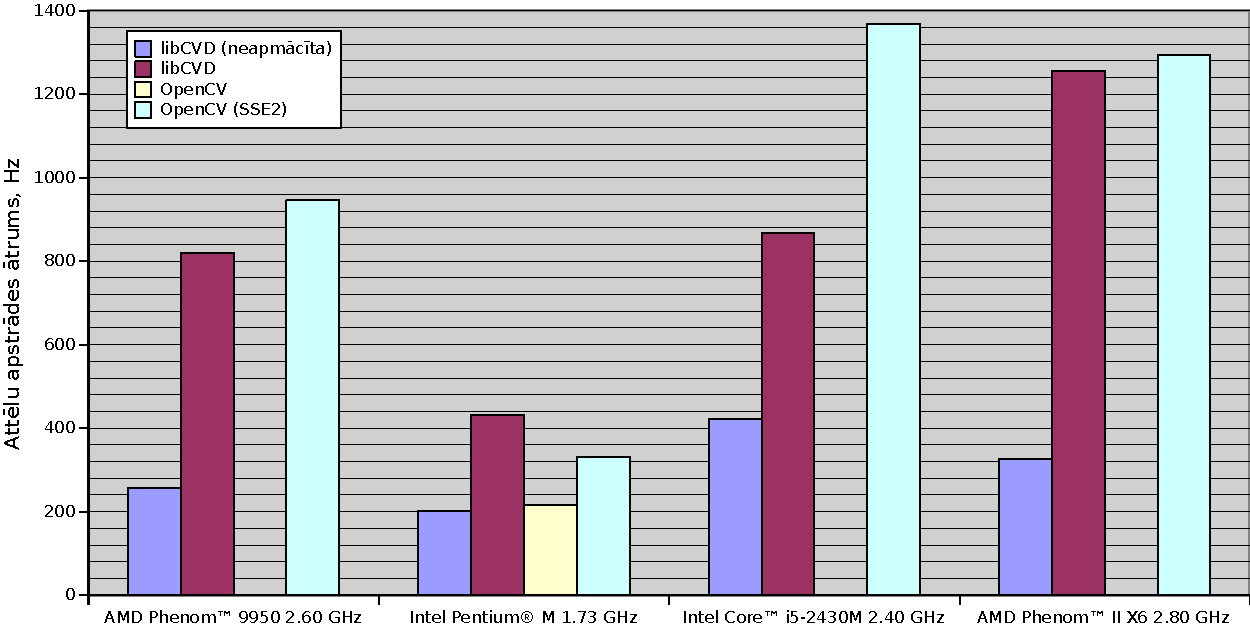
\includegraphics[width=\linewidth]{chart-cpu2}
	\caption{FAST CPU implementāciju ātrdarbības salīdzinājums.}
	\label{fig:test1-data-txt}
\end{figure}

Vecākas paaudzes Pentium procesoram labākais ātrdarbības rādītājs bija tieši
mašīnmācāmajai (libCVD) FAST implementācijai, savukārt jaunāko paaudžu
procesoriem labāku ātrdarbību uzrādīja OpenCV SSE2 uzlabotā implementācija.
AMD~Phenom~II gadījumā libCVD un OpenCV SSE2 implementācijas uzrādīja
līdzvērtīgu rezultātu.
Šādi rezultāti skaidrojami, galvenokārt, ar SSE2 veiktspējas uzlabojumiem
jauno paaudžu procesoriem~\cite{Core2}. Papildus tam, mašīnmācāmā FAST
implementācijas jautājumu koks veido apjomīgu mašīnkodu ar lielu skaitu
zarošanos. Koda apjoms un nelineārā izpildes secība samazina izpildes koda
lokalitāti un ierobežo instrukciju kešatmiņas efektivitāti.

\ref{fig:test1-data-txt}~attēlā OpenCV (bez SSE2) rezultāti 64~bitu
sistēmām nav uzrādīti, jo kompilācijas sistēma nerespektēja (ignorēja)
SSE2 atspējošanu un iegūtie rezultāti bija nekorekti
(\ref{fig:test1-data}~attēls \pageref{fig:test1-data}~lapā iekļauj arī nekorektos
rezultātus).

GPU implementācijas ātrdarbība tika salīdzināta ar CPU platformu,
kas uzrādīja līdzīgus rezultātus ar CPU implementāciju, bet tos
nepārsniedzot, kā tika paredzēts (sk.~\ref{fig:test2-data-txt}~att.).
Autors šo veiktspējas
ierobežojumu skaidro ar salīdzinoši mazo datu apjomu un
zemu nepieciešamo skaitļošanas apjomu. Tādējādi GPU straumes
procesori nav pietiekami piesātināti ar datiem, kā rezultātā tie
procentuāli daudz laika pavada dīkstāvē un
GPU augstais latentums ir galvenais ierobežojošais faktors.
(GPU arhitektūra apskatīta \ref{sec:gpu}~nodaļā).
\begin{figure}[tbh]
	\centering
	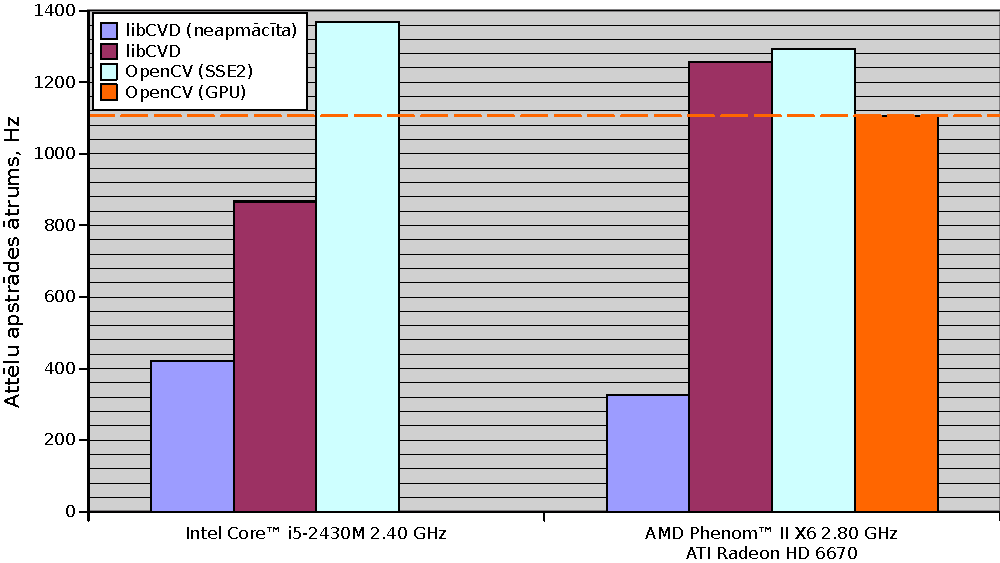
\includegraphics[scale=0.77]{chart-gpu2}
	\caption{FAST GPU un CPU implementāciju ātrdarbības salīdzinājums.}
	\label{fig:test2-data-txt}
\end{figure}

Autora izstrādātais FPGA implementācijas modelis tika sintezēts ar
dažādu skaitu punktu apstrādes vienību un to veiktspēja aprēķināta
ņemot vērā sintēzes rezultātos iegūto maksimālo frekvenci.
Testos novērots, ka $12 \times 12$ pikseļu gabala apstrāde pie
aptuveni $400\units{MHz}$ takts frekvences sasniedz CPU platformas
labākos rezultātus.
Rezultāti ilustrēti \ref{fig:test3-data-txt}~attēlā, kur ar
melnu, pārtrauktu līniju atzīmēts labākais
CPU implementācijas rezultāts. Ātrdarbība FPGA ir palielināma
instancējot vairāk punktu apstrādes vienību.

\begin{figure}[tbh]
	\centering
	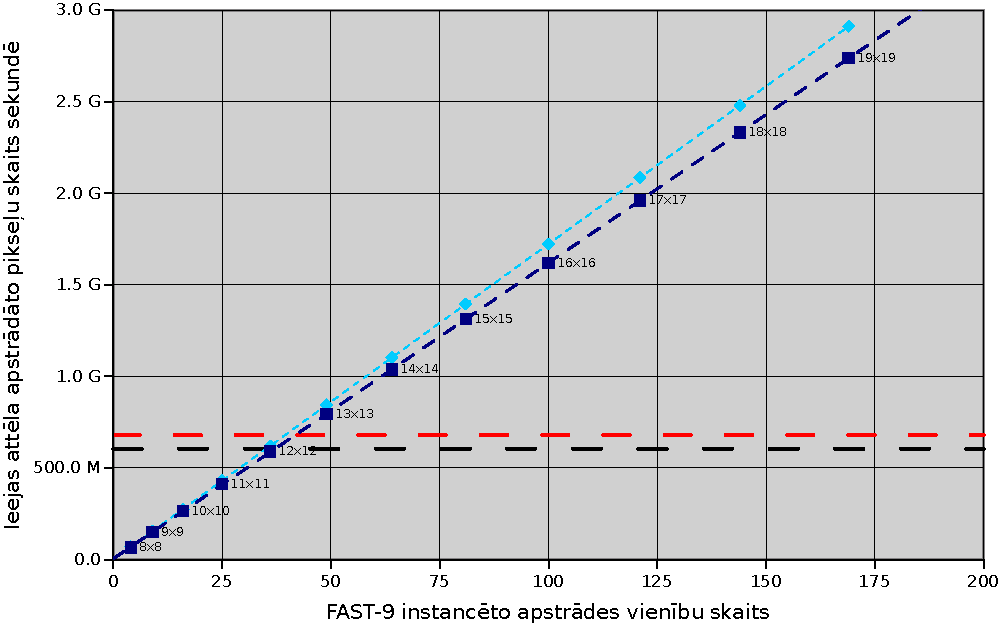
\includegraphics[scale=0.77]{chart-fpga}
	\caption{Pikseļu apstrādes ātrums pret \texttt{fast\_n\_unit} instanču skaitu.}
	\label{fig:test3-data-txt}
\end{figure}

Kopumā, FAST implementācija FPGA uzrādīja augstāko potenciālo ātrdarbību,
aiz kuras seko CPU. GPU uzrādīja līdzīgu rezultātu kā CPU, bet tests ar
vienu ierīci nevar adekvāti vispārēji atspoguļot GPU platformas veiktspēju.
Autors arī uzsver,
ka pat ja GPU implementācija uzrāda zemāku ātrdarbību nekā CPU, tā
izmantošana tomēr var palielināt kopējo (heterogēnas) sistēmas ātrdarbību
atslogojot CPU, gadījumos, ja tam jāveic papildus skaitļošanas uzdevumi.
Visu pārbaudīto ierīču ātrdarbība ievērojami pārsniedza
30~kadrus sekundē ($768 \times 576$ pikseļu lielam kadram) 
un tās ir izmantojamas reāllaika datu
straumes apstrādei. 30~kadri sekundē gan nav mērķis, bet minimums, jo
raksturpunktu detektēšana ir tikai viens solis, un lai nodrošinātu
pietiekamu apstrādes laiku visam uzdevumam, šis rādītājs ir jāpārsniedz
vairākas reizes.

